
%(BEGIN_QUESTION)
% Copyright 2010, Tony R. Kuphaldt, released under the Creative Commons Attribution License (v 1.0)
% This means you may do almost anything with this work of mine, so long as you give me proper credit

An instrument technician desires to simulate a thermocouple signal using a precision voltage reference and a voltage divider network of her own making:

$$\includegraphics[width=15.5cm]{i03738x01.eps}$$

Calculate the necessary value for resistor $R_1$ in order to generate a millivoltage signal simulating a type J thermocouple at 607 degrees Fahrenheit.  Assume the instrument receiving this signal has reference junction compensation enabled, and is at an ambient temperature of 71 degrees Fahrenheit.

\vskip 10pt

$R_1$ = \underbar{\hskip 50pt}

\vfil 

\underbar{file i03738}
\eject
%(END_QUESTION)





%(BEGIN_ANSWER)

This is a graded question -- no answers or hints given!

%(END_ANSWER)





%(BEGIN_NOTES)

Since we know the thermocouple instrument has reference junction compensation enabled, we know we must ``fool'' this instrument into thinking it has a real thermocouple reference junction to compensate for.  From our basic thermocouple circuit formula, showing the voltage received by any receiving instrument (e.g. a voltmeter) to be equal to the difference in junction voltages (measurement $-$ reference):

$$V_{inst} = V_{meas} - V_{ref}$$

We need to input to this instrument the same voltage it would receive with a type J measurement junction at 607 $^{o}$F (17.403 mV) and a type J reference junction at 71 $^{o}$F (1.105 mV).

$$V_{inst} = 17.403 \hbox{ mV} - 1.105 \hbox{ mV} = 16.298 \hbox{ mV}$$

\vskip 10pt

Therefore, resistor $R_2$ needs to drop 16.298 millivolts.  In order for this to happen, the 27 ohm resistor $R_2$ must carry a current equal to 0.6036 milliamps.  Given a total supply voltage of 2.5 volts, this necessitates a total circuit resistance of 4141.6 ohms.  Subtracting the 27 ohms of $R_2$, we are left with {\bf 4114.6 ohms} for $R_1$'s resistance.

%INDEX% Measurement, temperature: thermocouple

%(END_NOTES)

